\chapter{APPENDIX. In every life, explanations for technical terms are desirable at one period or another; and, such period may come during youth, or it may be delay- ed until advanced age. I find it impossible to write at length upon violin tone-peculiarities without employment of some technical terms; and, remem- bering the period when technical language was confusing to myself, and remembering my pleasure accompaning elucidation of such language, and, remembering my desire that all readers receive re- ward for the punishment incidental to wading through the dry details on preceeding pages, there- fore do I willingly append an explanation for some of the more confusing terms necessarily employed herein. To those readers not interested in such explanations, 'tis unnecessary to suggest the waste of time in reading these closing pages. ALT: All tones in the first octave above the}

\begin{figure}[h!]
\centering

\includegraphics[width=0.8\textwidth]{../imagenes/pagina_297_fig_01.png}
\caption{Figura de la página 297}
\end{figure}

\begin{figure}[h!]
\centering
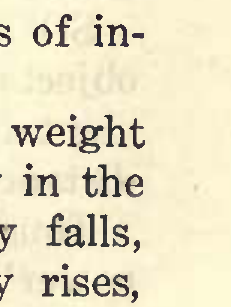
\includegraphics[width=0.8\textwidth]{../imagenes/pagina_297_fig_02.png}
\caption{Figura de la página 297}
\end{figure}

staff. ALTISSIMO: All tones above alt. METEORIC CONDITIONS: Are such condi- tions of the air as barometic pressure, temperature, humidity, (water vapor,) winds, and clouds. As all of these items, singly, or combined, operate to di- minish or augment the distance traveled by sound- waves, therefor, such items become matters of in- terest to the student of violin tone. BAROMETRIC PRESSURE: Refers to weight of the air as indicated by action of mercury in the tube of the barometer. As the mercury falls, weight of air is lighter. As the mercury rises,

289

\begin{figure}[h!]
\centering
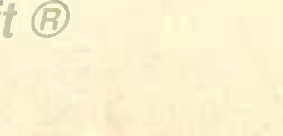
\includegraphics[width=0.8\textwidth]{../imagenes/pagina_298_fig_01.png}
\caption{Figura de la página 298}
\end{figure}

\begin{figure}[h!]
\centering

\includegraphics[width=0.8\textwidth]{../imagenes/pagina_298_fig_02.png}
\caption{Figura de la página 298}
\end{figure}

\begin{figure}[h!]
\centering

\includegraphics[width=0.8\textwidth]{../imagenes/pagina_298_fig_03.png}
\caption{Figura de la página 298}
\end{figure}

\section{VIOLIN TONE-PECULIARITIES.}

weight of air is heavier. Such variations in the weight of air are frequent, especially in our sum- mer months, and, they may be so great as to cause great difference in the distance traveled by any sound from any source whatever. Strangely, the violin, of all musical devices, is the most sensitive to atmospheric conditions as is manifested by feebleness of tone-inten sity upon dates when heat and water vapor are in excess. Under such con- ditions, string-tone values suffer unavoidable de- preciation, no matter who the maker, nor what the quality of material. THE NIMBUS CLOUD: Overspreading all of the sky, operates to augment distance traveled by sound-waves. TEMPERATURE: May be either so high, or low as to greatly diminish the distance traveled by sound-waves. WINDS: Operate to diminish the distance trav- eled by sound-waves in opposition, to the current, and, to augment the distance traveled with the current. HOUR OF DAY: Is of importance in the record for the distance traveled by sound-waves, because during the midday hours, sound is propagated with greatest difficulty upon any given day. SOUND-REFLECTING AGENTS: Are such objects as buildings, hills, timber, operating to aug- ment distance traveled by violin tone in the long- distance out-of-doors test for intensity. Thus, the record of any violin for "carrying power "possesses but little interest unless accompa-

290

\begin{figure}[h!]
\centering
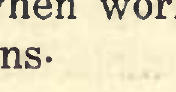
\includegraphics[width=0.8\textwidth]{../imagenes/pagina_299_fig_01.png}
\caption{Figura de la página 299}
\end{figure}

\begin{figure}[h!]
\centering
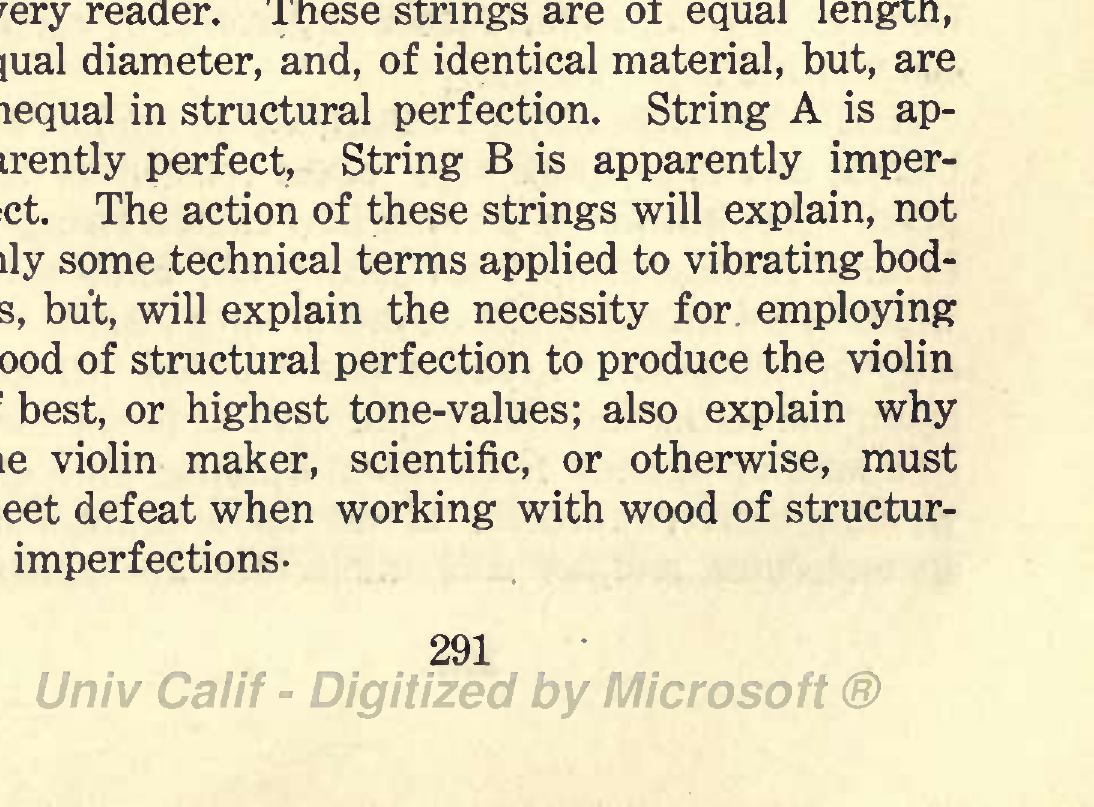
\includegraphics[width=0.8\textwidth]{../imagenes/pagina_299_fig_02.png}
\caption{Figura de la página 299}
\end{figure}

\begin{figure}[h!]
\centering
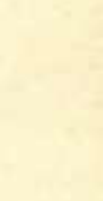
\includegraphics[width=0.8\textwidth]{../imagenes/pagina_299_fig_03.png}
\caption{Figura de la página 299}
\end{figure}

\begin{figure}[h!]
\centering
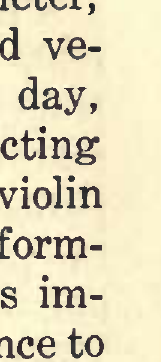
\includegraphics[width=0.8\textwidth]{../imagenes/pagina_299_fig_04.png}
\caption{Figura de la página 299}
\end{figure}

\begin{figure}[h!]
\centering
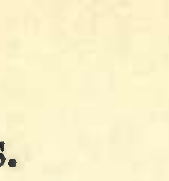
\includegraphics[width=0.8\textwidth]{../imagenes/pagina_299_fig_05.png}
\caption{Figura de la página 299}
\end{figure}

\begin{figure}[h!]
\centering
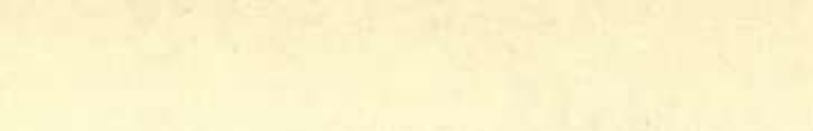
\includegraphics[width=0.8\textwidth]{../imagenes/pagina_299_fig_06.png}
\caption{Figura de la página 299}
\end{figure}

\section{VIOLIN TONE-PECULIARITIES.}

nied by the readings of the barometer, hygrometer, thermometer, together with the direction and ve- locity of winds, degree of cloudiness, hour of day, and, the presence or absence of sound-reflecting agents. With such record thus complete, a violin may be safely .guaranteed to repeat its perform- ance under similar meteoric conditions. It is im- portant to the violin player to know the distance to which the tone of his violin travels with ease. Thus, the player may avoid overexertion with the bow, as such overexertion always produces a dis- agreeable effect upon the musically cultivated ear. OSCILLATION, AMPLITUDE of OSCILLA- TION, VIBRATION, both NORMAL and TAN- GENTIAL, NODES, VENTRAL SEGMENTS, HARMONIC OVERTONES, and DISSONANT OVERTONES: Are explained thus: Confining this matter to facts of practical value to violin tone, I employ these two strings as a means for assistance in making definitions clear to the understanding of every reader. These strings are of equal length, equal diameter, and, of identical material, but, are A unequal in structural perfection. String is ap- parently perfect, String B is apparently imper- fect. The action of these strings will explain, not only some technical terms applied to vibrating bod- ies, but, will explain the necessity for employing wood of structural perfection to produce the violin of best, or highest tone- values; also explain why the violin maker, scientific, or otherwise, must meet defeat when working with wood of structur- al imperfections-

291

\begin{figure}[h!]
\centering

\includegraphics[width=0.8\textwidth]{../imagenes/pagina_300_fig_01.png}
\caption{Figura de la página 300}
\end{figure}

\begin{figure}[h!]
\centering

\includegraphics[width=0.8\textwidth]{../imagenes/pagina_300_fig_02.png}
\caption{Figura de la página 300}
\end{figure}

\section{VIOLIN TONE-PECULIARITIES.}

A motionless body is said to be at the point of rest. When a body moves to a certain distance from the point of rest, thence returns to the point of rest, thence passes to an equal distance in the op- posite direction, thence returns a second time to the point of rest, such body is said to be in vibrat- ion, or, in oscillation, whichever term is peferred. The distance traveled by such body from its point of rest is the amplitude of its oscillation. [It is of interest to note the fact that English and German philosophers differ with: French phil- osophers as to what movement of a vibrating body completes one vibration. The former hold that one complete vibration consists in one complete movement each way from the point of rest; where- as, the latter hold that one movement from the point of rest with one return completes one vibra- tion. Thus, from the French method of express- ion, concert pitch is given as A equals 900 vibrat- ions per second; whereas, from the English and German method, concert pitch is given as A equals 450 vibrations per second.] Attaching these strings separately to immovable blocks, and to separate pegs, equal tension is ap- plied. Application of a violin bow causes string A to wind rapidly around its long axis; and,, such winding continues in one direction until elastic en- ergy in string-fiber exceeds bow-friction; where- upon, the string unwinds itself, only to be instant- ly wound up again. Such rapid winding and un- winding delivers forceful blows upon contiguous air molecules, and, as such molecules are elastic

292

\begin{figure}[h!]
\centering
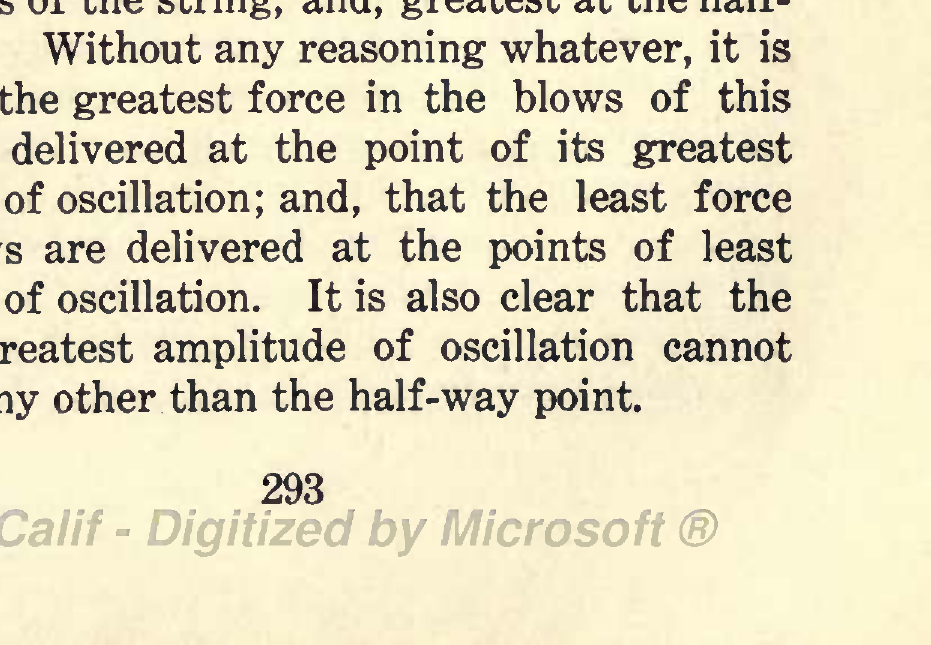
\includegraphics[width=0.8\textwidth]{../imagenes/pagina_301_fig_01.png}
\caption{Figura de la página 301}
\end{figure}

\begin{figure}[h!]
\centering
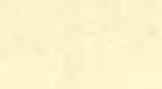
\includegraphics[width=0.8\textwidth]{../imagenes/pagina_301_fig_02.png}
\caption{Figura de la página 301}
\end{figure}

\begin{figure}[h!]
\centering
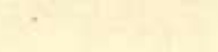
\includegraphics[width=0.8\textwidth]{../imagenes/pagina_301_fig_03.png}
\caption{Figura de la página 301}
\end{figure}

\section{VIOLIN TONE-PECULIARITIES.}

spheres, and, as such spheres touch each other, therefore, the blows from the string arouse sound- wave movement; and; as such movement reaches our tympani, (ear drums, ) we become conscious of a tone proceeding from the string; and, as such tone is produced by action of the entire length of the string, therefore this tone is of the lowest pos- sible pitch for a string of this length, and, with this tension; therefore this tone is the fundament- al tone of string A. [Although this tone is fundamental to string A, yet, we may not suppose that no other fundament- al tone can be produced upon string A, because, when shortening the string by "stopping" it, as with pressure of the finger, a new tone of higher pitch is produced; and such new tone may be rightfully called the fundamental tone of a new key; and, the same holds true of all other tones of higher pitch.] The action of string A, at once causes the ap- pearance of absorbing phenomena; one of which consists in the string describing a circle around its long axis. We observe that such circle is smallest at the ends of the string, and, greatest at the half- way point. Without any reasoning whatever, it is clear that the greatest force in the blows of this string are delivered at the point of its greatest amplitude of oscillation; and, that the least force in its blows are delivered at the points of least amplitude of oscillation. It is also clear that the point of greatest amplitude of oscillation cannot occur at any other than the half-way point.

293

\begin{figure}[h!]
\centering
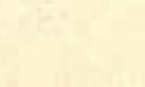
\includegraphics[width=0.8\textwidth]{../imagenes/pagina_302_fig_01.png}
\caption{Figura de la página 302}
\end{figure}

\begin{figure}[h!]
\centering

\includegraphics[width=0.8\textwidth]{../imagenes/pagina_302_fig_02.png}
\caption{Figura de la página 302}
\end{figure}

\begin{figure}[h!]
\centering
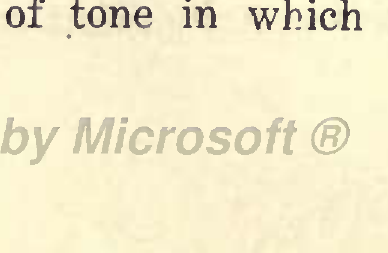
\includegraphics[width=0.8\textwidth]{../imagenes/pagina_302_fig_03.png}
\caption{Figura de la página 302}
\end{figure}

\begin{figure}[h!]
\centering
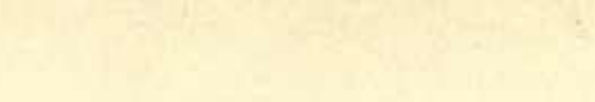
\includegraphics[width=0.8\textwidth]{../imagenes/pagina_302_fig_04.png}
\caption{Figura de la página 302}
\end{figure}

\section{VIOLIN TONE-PECULIARITIES.}

[Acting upon this fact, when graduating the sounding-board for maximum tone-power, thick- ness, from bridge-position and from the ends of the plate, slightly diminishes to the half-way point; and, for the purpose of increasing the am- plitude of oscillation at such point. From the action of the string, it is clear that equal amplitude of oscillation cannot be secured at any other point between bridge-position and the ends of the plate. Another phenomena, observed upon string A, di- rects attention to nodes, ventral segments and harmonic overtones. Lightly stopping the string at the half-way point, in either direction therefrom are seen several points where the string is at rest. These points of rest are called nodes. They are equally distant from each other, and the space between two nodes is called a ventral seg- ment; and, we observe that each ventral segment acts precisely as the whole length of the string acts; that is, the widest amplitude of ventral seg- ment oscillation is at its half-way point; and, that the action of these ventral segments produces a musical tone. As the ventral segments are of sim- ilar length, therefore the tone of each segment is of the same pitch as the tone of its neighbor: and, as the pitch of such tone is in harmony with the fundamental tone, therefore such tone is called a harmonic overtone, and joining with the fundament- al tone, produces what is called "rich" tone a rare quality of tone a quality of tone highly valued by the violin soloist a quality of tone in which no

294

\begin{figure}[h!]
\centering

\includegraphics[width=0.8\textwidth]{../imagenes/pagina_303_fig_01.png}
\caption{Figura de la página 303}
\end{figure}

\begin{figure}[h!]
\centering
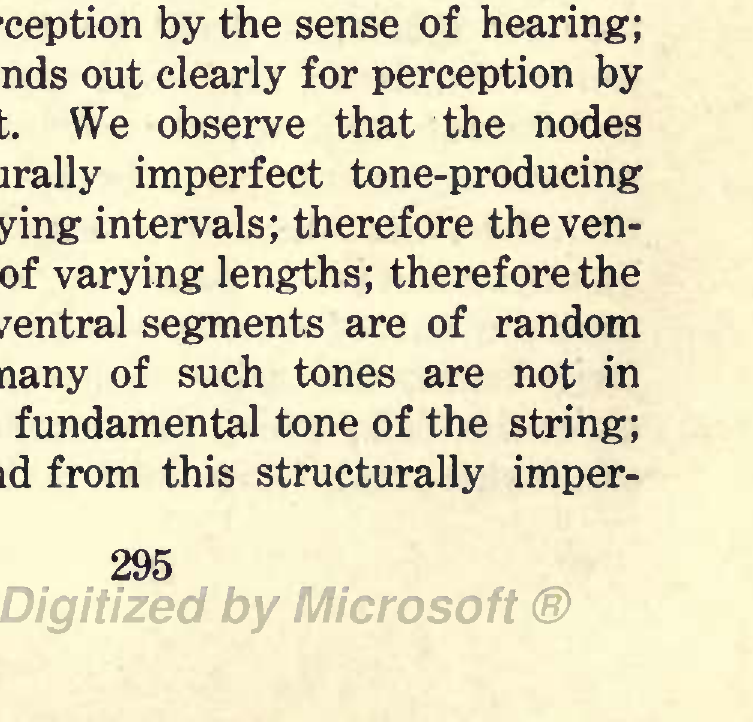
\includegraphics[width=0.8\textwidth]{../imagenes/pagina_303_fig_02.png}
\caption{Figura de la página 303}
\end{figure}

\begin{figure}[h!]
\centering
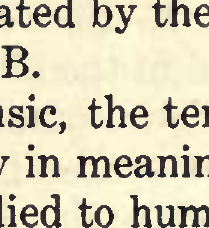
\includegraphics[width=0.8\textwidth]{../imagenes/pagina_303_fig_03.png}
\caption{Figura de la página 303}
\end{figure}

\begin{figure}[h!]
\centering
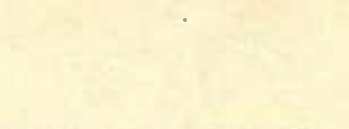
\includegraphics[width=0.8\textwidth]{../imagenes/pagina_303_fig_04.png}
\caption{Figura de la página 303}
\end{figure}

\section{VIOLIN TONE-PECULIARITIES.}

other musical device approaches the "best" violin a quality of tone impossible to the sounding- board of structural imperfections; and, the reason will be demonstrated by the action of structurally imperfect string B. [Applied to music, the terms "consonant," and, "dissonant" vary in meaning as widely as "saint" and "devil" applied to humanity. Consonant har- monic overtones, and, harmonics a basso, are the causes for enchanting beauty of violin tone. They lie between such terms as "sweetness," and, "richness." To them we are indebted for the crown which we so enthusiastically offer to "The King." But, we are reminded, very of ten remind- ed, that there are other crowns. Satan wears one. Strangely, Satan's crown may come from the vio- lin; and yet more strange, Satan's activity in cornering material for his crown is supplemented by such SCIENTIFIC violin makers who ignore structural perfection in sounding-board wood.] Applying the bow to string B, the dissonant overtone, (chief gem in Satan's crown,) stands out clearly for perception by the sense of hearing; and, the cause stands out clearly for perception by the sense of sight. We observe that the nodes upon this structurally imperfect tone-producing agent exist at varying intervals; therefore the ven- tral segments are of varying lengths; therefore the tones from these ventral segments are of random pitch; therefore many of such tones are not in harmony with the fundamental tone of the string; therefore the sound from this structurally imper-

295

\begin{figure}[h!]
\centering
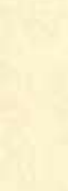
\includegraphics[width=0.8\textwidth]{../imagenes/pagina_304_fig_01.png}
\caption{Figura de la página 304}
\end{figure}

\begin{figure}[h!]
\centering
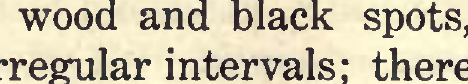
\includegraphics[width=0.8\textwidth]{../imagenes/pagina_304_fig_02.png}
\caption{Figura de la página 304}
\end{figure}

\begin{figure}[h!]
\centering
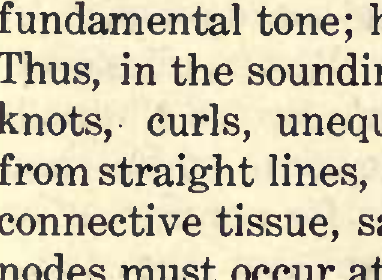
\includegraphics[width=0.8\textwidth]{../imagenes/pagina_304_fig_03.png}
\caption{Figura de la página 304}
\end{figure}

\begin{figure}[h!]
\centering
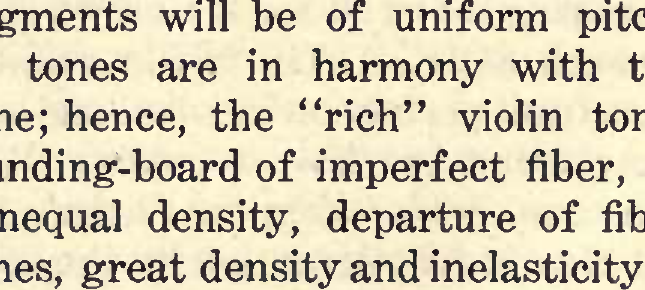
\includegraphics[width=0.8\textwidth]{../imagenes/pagina_304_fig_04.png}
\caption{Figura de la página 304}
\end{figure}

\begin{figure}[h!]
\centering
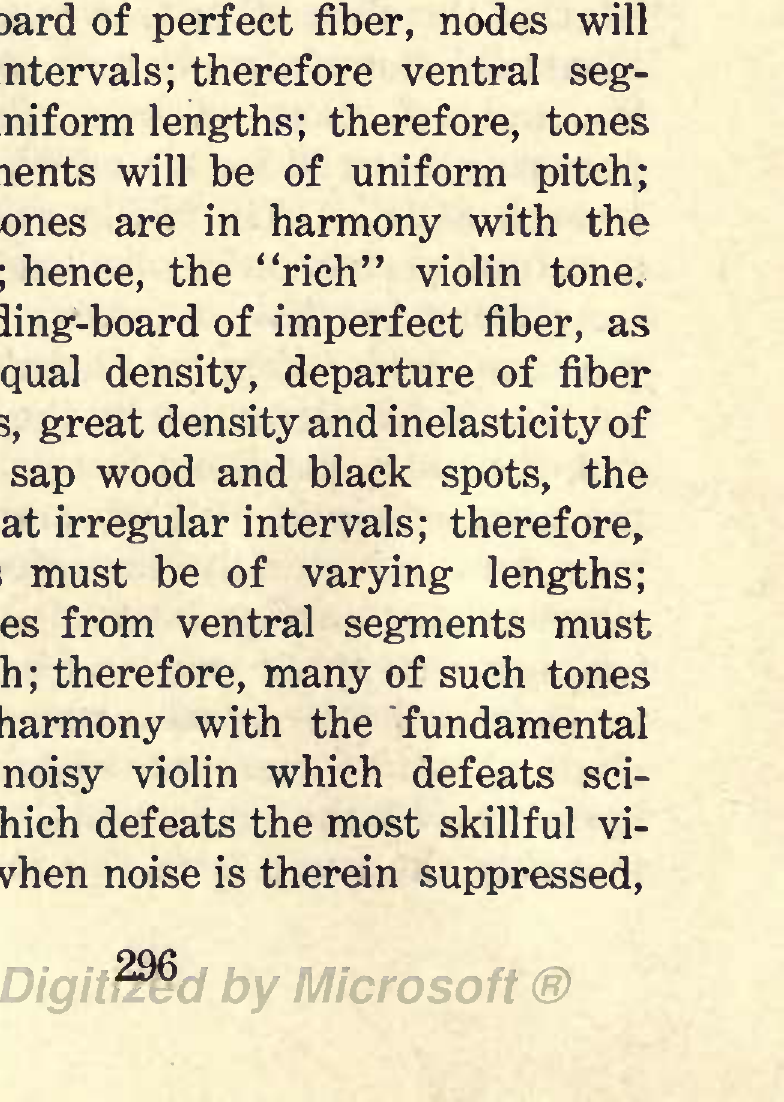
\includegraphics[width=0.8\textwidth]{../imagenes/pagina_304_fig_05.png}
\caption{Figura de la página 304}
\end{figure}

\begin{figure}[h!]
\centering
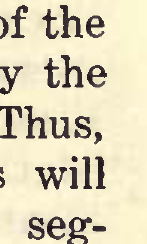
\includegraphics[width=0.8\textwidth]{../imagenes/pagina_304_fig_06.png}
\caption{Figura de la página 304}
\end{figure}

\begin{figure}[h!]
\centering
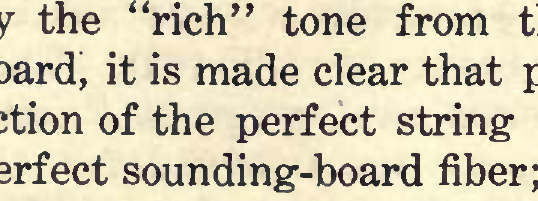
\includegraphics[width=0.8\textwidth]{../imagenes/pagina_304_fig_07.png}
\caption{Figura de la página 304}
\end{figure}

\begin{figure}[h!]
\centering
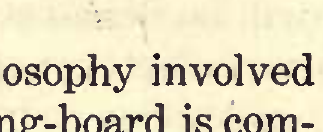
\includegraphics[width=0.8\textwidth]{../imagenes/pagina_304_fig_08.png}
\caption{Figura de la página 304}
\end{figure}

\begin{figure}[h!]
\centering
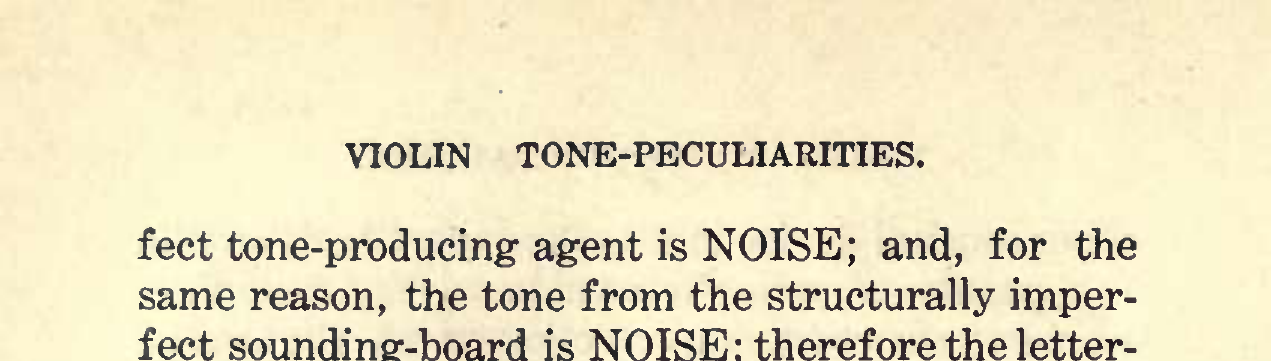
\includegraphics[width=0.8\textwidth]{../imagenes/pagina_304_fig_09.png}
\caption{Figura de la página 304}
\end{figure}

\section{VIOLIN TONE-PECULIARITIES.}

feet tone-producing agent is NOISE; and, for the same reason, the tone from the structurally imper- fect sounding-board is NOISE; therefore the letter- ing on Satan's crown is N-0-I-S-E. In text books devoted to the philosophy involved in musical sound, the violin sounding-board is com- pared with a "bundle of strings;" and, determin- ing by the "rich" tone from the perfect string, and, by the "rich" tone from the perfect sounding- board, it is made clear that part of the vibratory action of the perfect string is duplicated by the perfect sounding-board fiber; also, that part of the action of the imperfect string is duplicated by the action of the imperfect sounding-board fiber. Thus, in the sounding-board of perfect fiber, nodes will occur at regular intervals; therefore ventral seg- ments will be of uniform lengths; therefore, tones from ventral segments will be of uniform pitch; therefore, such tones are in harmony with the fundamental tone; hence, the "rich" violin tone. Thus, in the sounding-board of imperfect fiber, as knots, curls, unequal density, departure of fiber from straight lines, great density and inelasticity of connective tissue, sap wood and black spots, the nodes must occur at irregular intervals; therefore, ventral segments must be of varying lengths; therefore, the tones from ventral segments must be of random pitch therefore, many of such tones must be out of harmony ; with the fundamental tone; hence, the noisy violin which defeats sci- ence; the violin which defeats the most skillful vi- olin maker; and, when noise is therein suppressed,

296

\section{VIOLIN TONE-PECULIARITIES.}

'tis the violin of "cold" tone; and the violin of "cold" tone is no longer "The King." VIBRATORY MOVEMENT: In the violin sounding-board command deep interest from the student; and, such interest 'is due to the fact that, with other factors at the best, violin tone-values depend upon both normal vibratory movement, which travels along the fibers, and, tangential vi- bratory movement, which travels across the fibers. These two vibratory movements are the very foundation of violin tone-values. They are the factors which augment the tone of the strings. Without these factors,, violin tone- values depreciate to the level of the "broom-stick fiddle." By the presence of dry sand upon the flat sounding-board, both normal and tangential vibratory movements become defined. Uniformly distributed upon such sounding-board, the sand is thrown upward by the force of plate-oscillation; and, is thrown up to a height proportionate to the amplitude of such os- cillation. Right here is where we observe astound- ing variations in the spring-action of different samples of wood. Right here also is shown the vast difference between the action of the structur- ally perfect and imperfect fiber. Thus: Upon the perfect sounding-board, oscillation thereof, and continued during a period of time varying as the spring-action, forces the sand to leave ventral seg- ments, and, to collect upon the nodes. Thus, reg- ularity in the distance between nodes is determ- ined. Thus, irregularity in the distance between nodes is shown .on the structurally imperfect

297

\begin{figure}[h!]
\centering
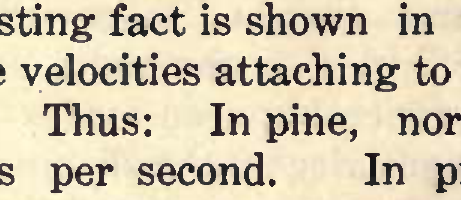
\includegraphics[width=0.8\textwidth]{../imagenes/pagina_306_fig_01.png}
\caption{Figura de la página 306}
\end{figure}

\begin{figure}[h!]
\centering
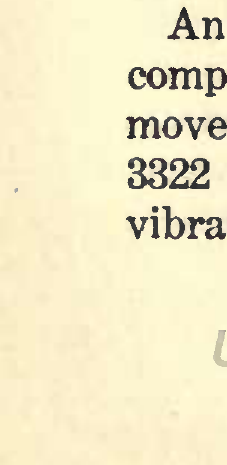
\includegraphics[width=0.8\textwidth]{../imagenes/pagina_306_fig_02.png}
\caption{Figura de la página 306}
\end{figure}

\begin{figure}[h!]
\centering
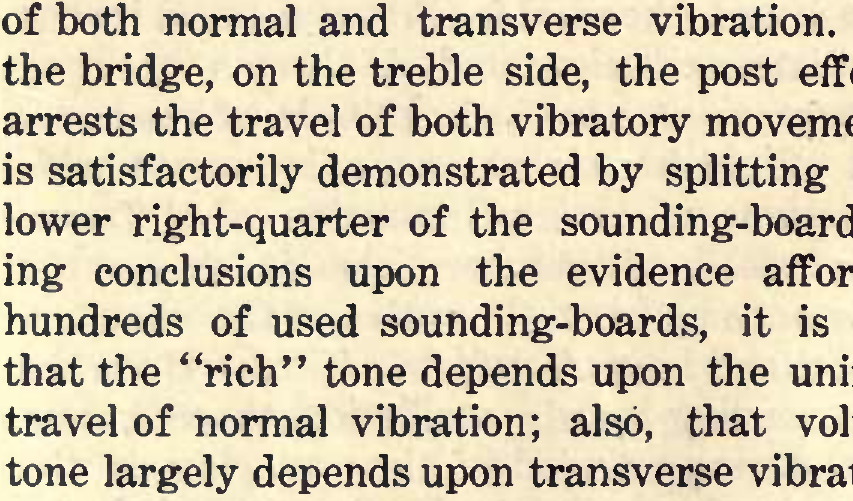
\includegraphics[width=0.8\textwidth]{../imagenes/pagina_306_fig_03.png}
\caption{Figura de la página 306}
\end{figure}

\begin{figure}[h!]
\centering
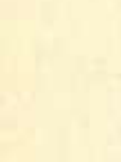
\includegraphics[width=0.8\textwidth]{../imagenes/pagina_306_fig_04.png}
\caption{Figura de la página 306}
\end{figure}

\begin{figure}[h!]
\centering
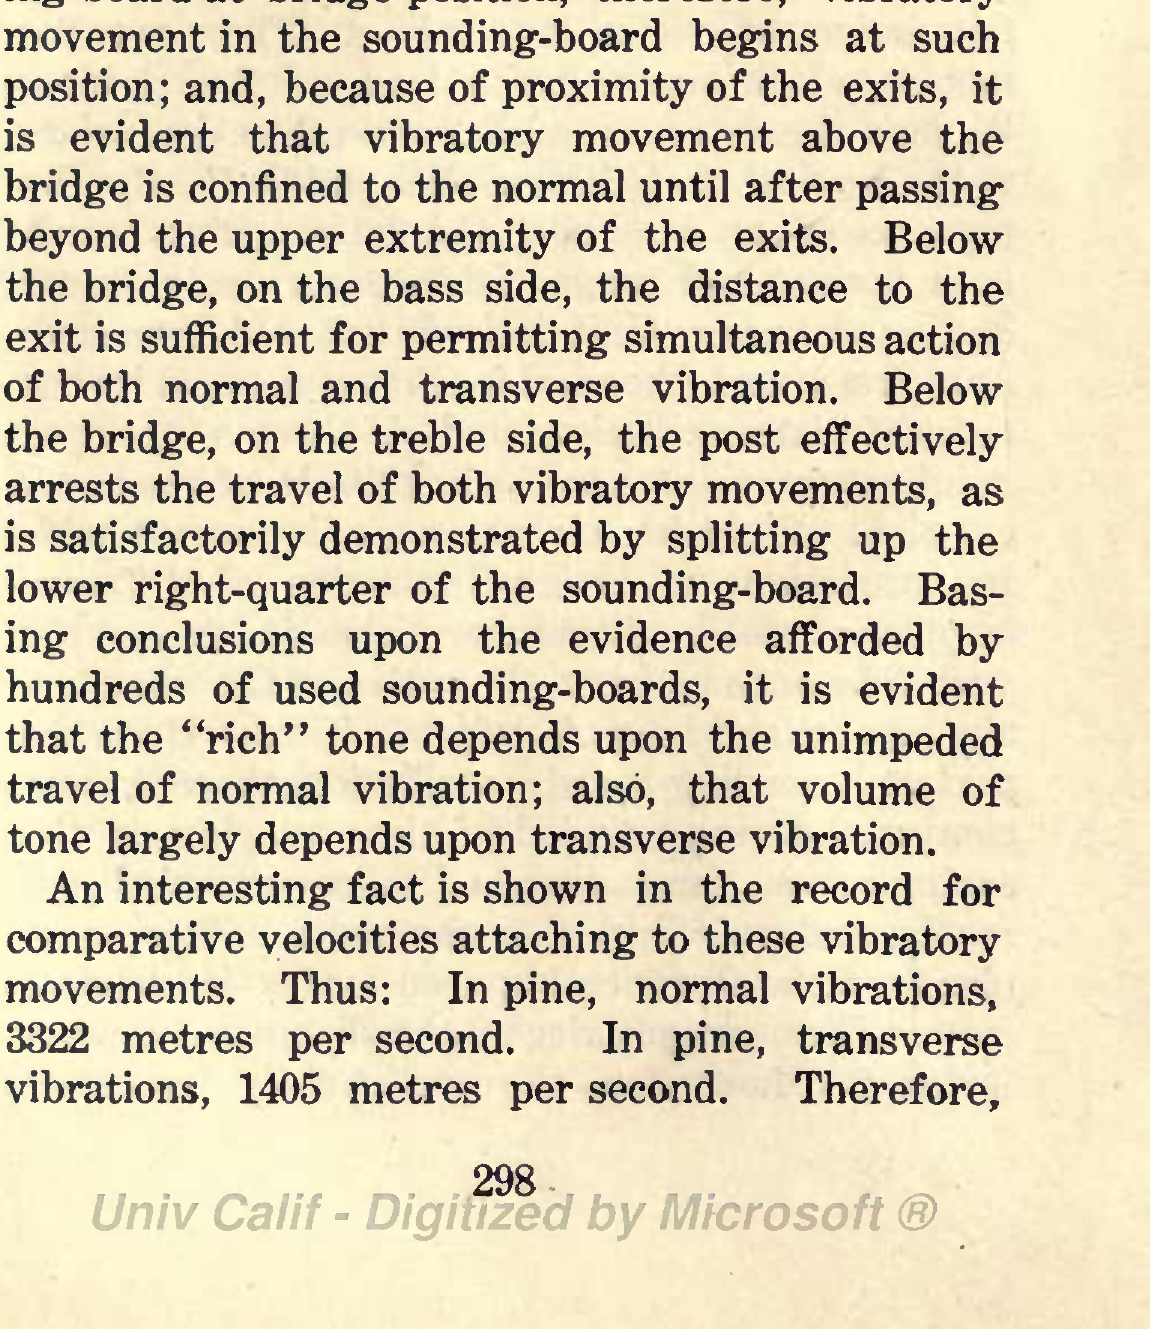
\includegraphics[width=0.8\textwidth]{../imagenes/pagina_306_fig_05.png}
\caption{Figura de la página 306}
\end{figure}

\begin{figure}[h!]
\centering
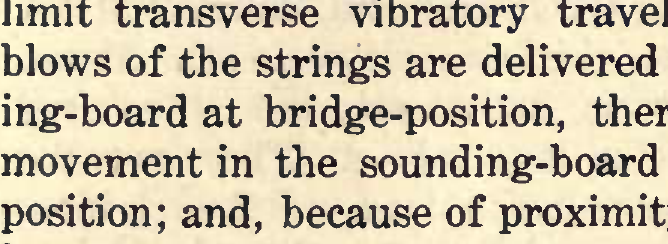
\includegraphics[width=0.8\textwidth]{../imagenes/pagina_306_fig_06.png}
\caption{Figura de la página 306}
\end{figure}

\begin{figure}[h!]
\centering
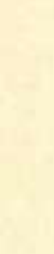
\includegraphics[width=0.8\textwidth]{../imagenes/pagina_306_fig_07.png}
\caption{Figura de la página 306}
\end{figure}

\begin{figure}[h!]
\centering
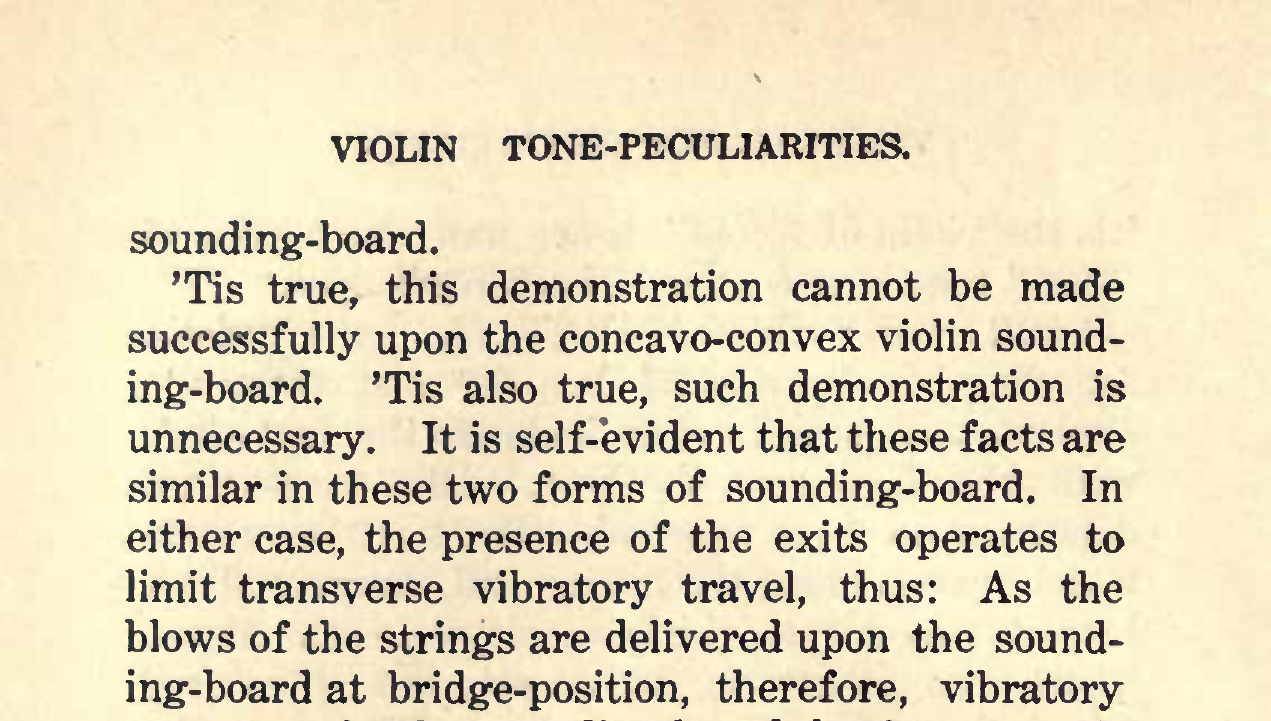
\includegraphics[width=0.8\textwidth]{../imagenes/pagina_306_fig_08.png}
\caption{Figura de la página 306}
\end{figure}

\section{VIOLIN TONE-PECULIARITIES.}

sounding-board. 'Tis true, this demonstration cannot be made successfully upon the concavo-convex violin sound- ing-board. 'Tis also true, such demonstration is unnecessary. It is self-evident that these facts are similar in these two forms of sounding-board. In either case, the presence of the exits operates to limit transverse vibratory travel, thus: As the blows of the strings are delivered upon the sound- ing-board at bridge-position, therefore, vibratory movement in the sounding-board begins at such position; and, because of proximity of the exits, it is evident that vibratory movement above the bridge is confined to the normal until after passing beyond the upper extremity of the exits. Below the bridge, on the bass side, the distance to the exit is sufficient for permitting simultaneous action of both normal and transverse vibration. Below the bridge, on the treble side, the post effectively arrests the travel of both vibratory movements, as is satisfactorily demonstrated by splitting up the lower right-quarter of the sounding-board. Bas- ing conclusions upon the evidence afforded by hundreds of used sounding-boards, it is evident that the "rich" tone depends upon the unimpeded travel of normal vibration; also, that volume of tone largely depends upon transverse vibration. An interesting fact is shown in the record for comparative velocities attaching to these vibratory movements. Thus: In pine, normal vibrations, 3322 metres per second. In pine, transverse vibrations, 1405 metres per second. Therefore,

298

\begin{figure}[h!]
\centering
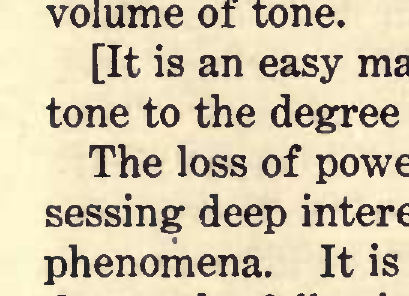
\includegraphics[width=0.8\textwidth]{../imagenes/pagina_307_fig_01.png}
\caption{Figura de la página 307}
\end{figure}

\section{VIOLIN TONE-PECULIARITIES.}

as transverse vibration travels one unit, nor- mal vibration travels 2 36-100 units; but, the evidence from used sounding-boards indicates that this ratio is not a constant quantity, that it is a quantity greatly modified by structural peculiar- ities of grain in different samples of wood. Thus, transverse vibration is dimished by both extremely soft grain, and extremely dense grain. United, these vibratory movements become the foundation of both volume of tone, and quality of tone. In the production of volume of tone from the sounding-board, transverse vibration exercises the more commanding influence. This fact is eas- ily demonstrated, thus: With that sounding-board too rigid for the force in strings of certain size, as gauge-2, gradual diminution of thickness from center join to edges operates to increase the distance traveled by transverse vibration; therefore, the area of the striking surface is increased; therefore, an increased number of air molecules within the violin body receive an identical blow; hence greater volume of tone. [It is an easy matter to increase volume of violin tone to the degree ruining intensity of tone.] The loss of power following use is a matter pos- sessing deep interest to the student of violin tone- phenomena. It is my observation that such loss is due to the following factors: 1. Increasing roughness of unprotected interior surfaces. 2. Disintegration upon unprotected surface. 3. Increasing sounding-board flexibility follow-

299

\begin{figure}[h!]
\centering
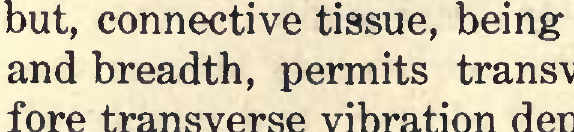
\includegraphics[width=0.8\textwidth]{../imagenes/pagina_308_fig_01.png}
\caption{Figura de la página 308}
\end{figure}

\begin{figure}[h!]
\centering
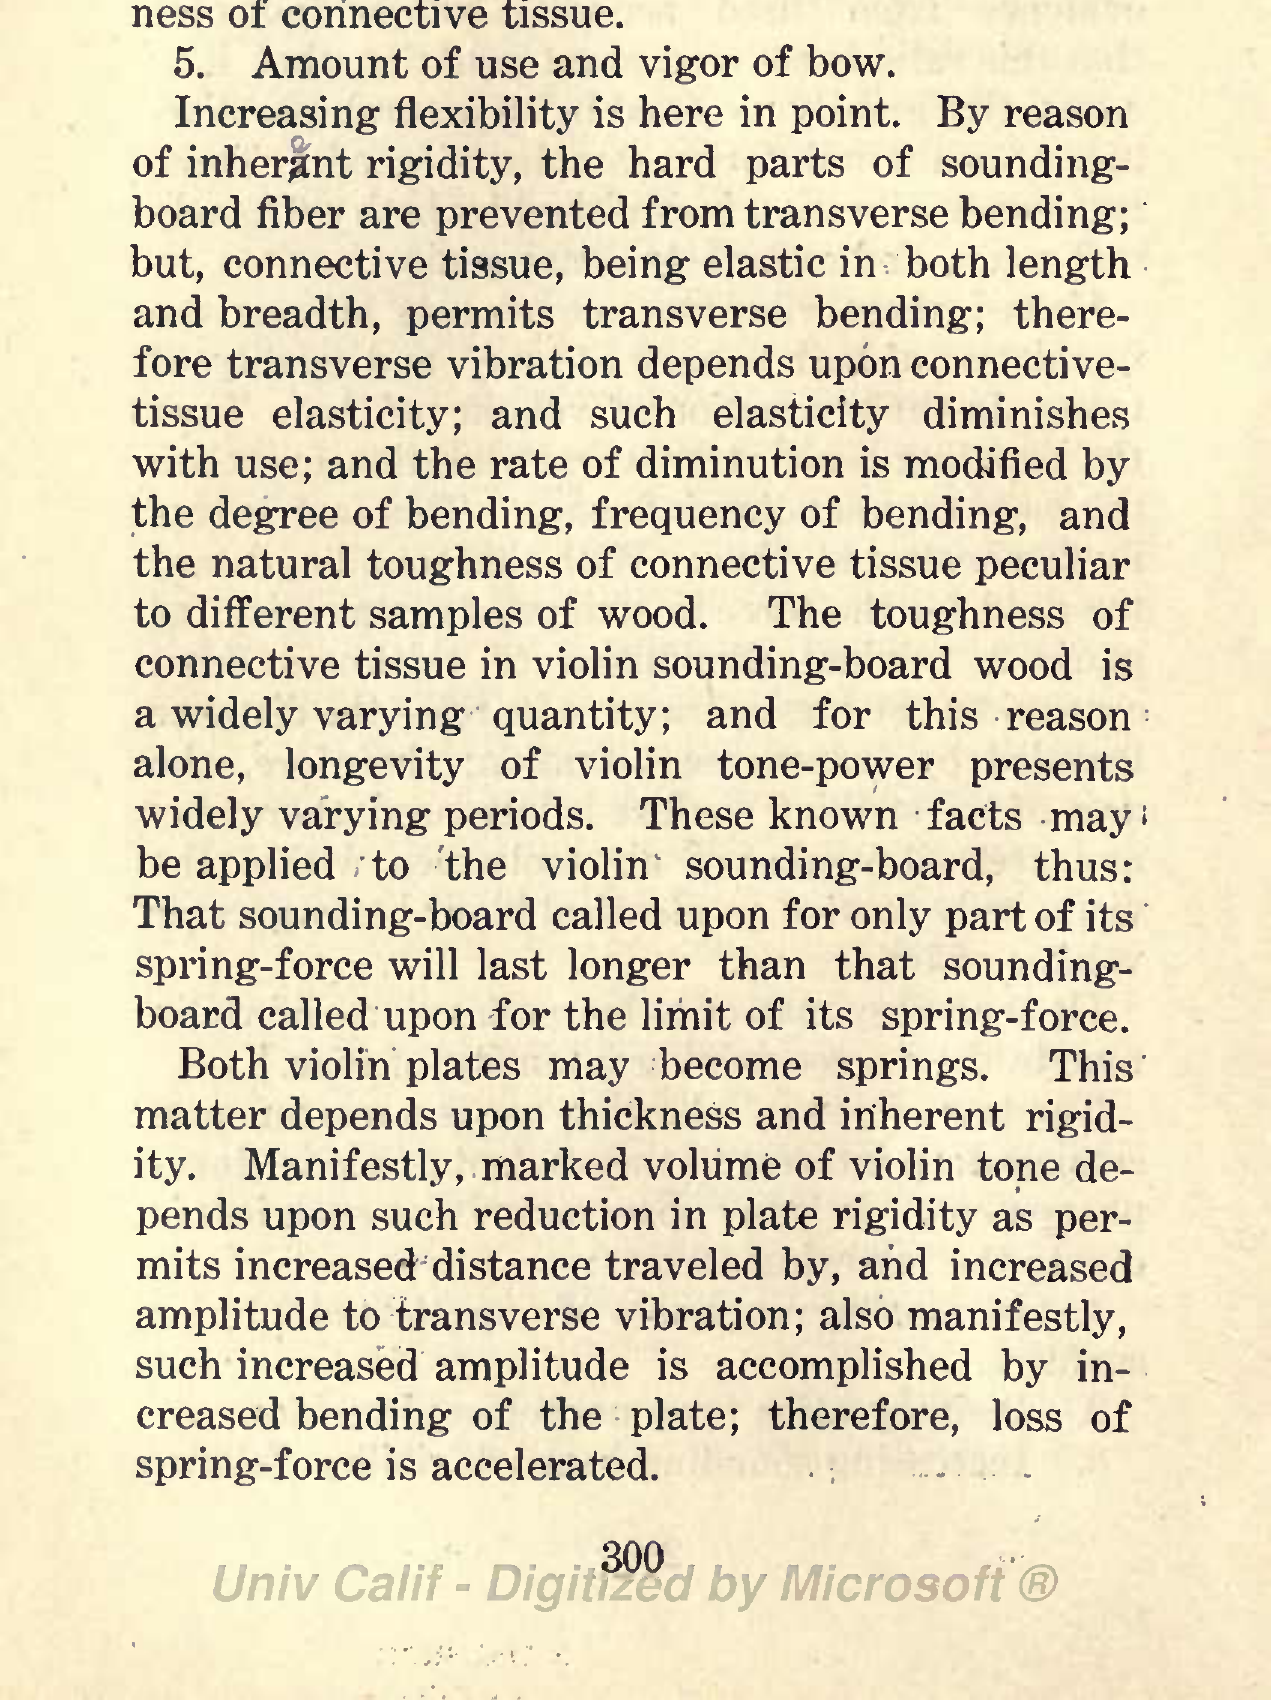
\includegraphics[width=0.8\textwidth]{../imagenes/pagina_308_fig_02.png}
\caption{Figura de la página 308}
\end{figure}

\begin{figure}[h!]
\centering
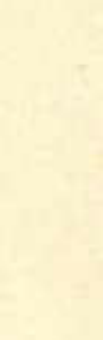
\includegraphics[width=0.8\textwidth]{../imagenes/pagina_308_fig_03.png}
\caption{Figura de la página 308}
\end{figure}

\begin{figure}[h!]
\centering
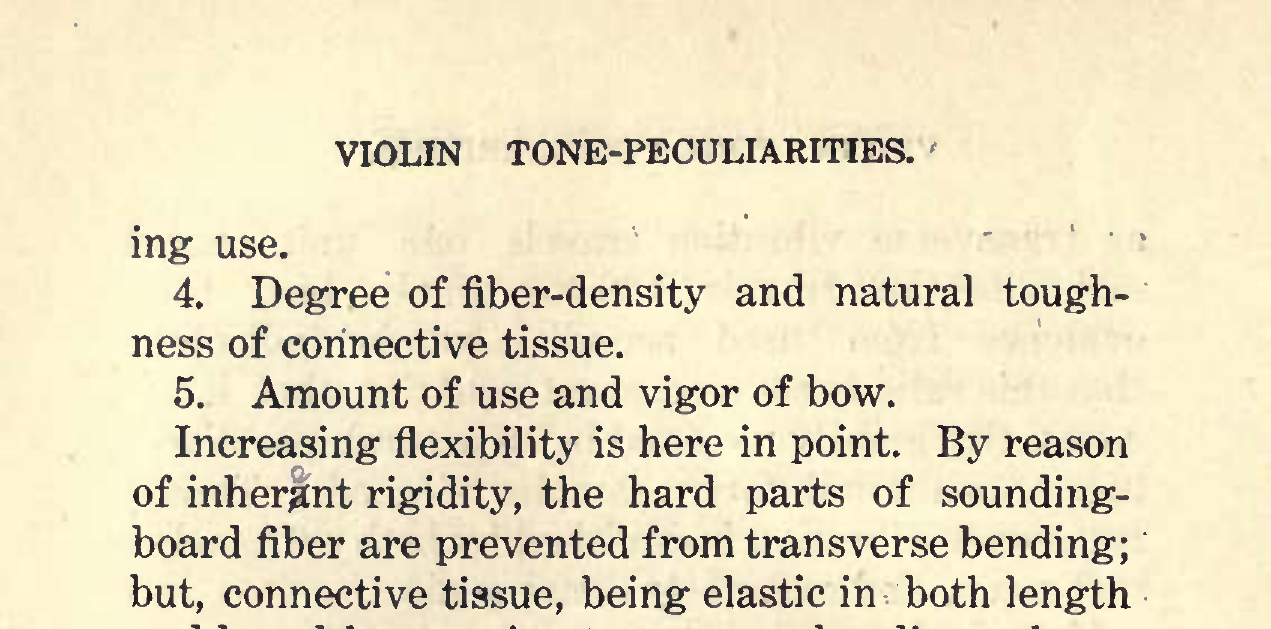
\includegraphics[width=0.8\textwidth]{../imagenes/pagina_308_fig_04.png}
\caption{Figura de la página 308}
\end{figure}

\section{VIOLIN TONE-PECULIARITIES.}

ing use. 4. Degree of fiber-density and natural tough- ness of connective tissue. 5. Amount of use and vigor of bow. Increasing flexibility is here in point. By reason of inherent rigidity, the hard parts of sounding- board fiber are prevented from transverse bending; but, connective tissue, being elastic in both length and breadth, permits transverse bending; there- fore transverse vibration depends upon connective- tissue elasticity; and such elasticity diminishes with use; and the rate of diminution is modified by the degree of bending, frequency of bending, and the natural toughness of connective tissue peculiar to different samples of wood. The toughness of connective tissue in violin sounding-board wood is a widely varying quantity; and for this reason alone, longevity of violin tone-power presents widely varying periods. These known facts may' be applied to the violin sounding-board, thus: That sounding-board called upon for only part of its spring-force will last longer than that sounding- board called upon for the limit of its spring-force. Both violin plates may become springs. This matter depends upon thickness and inherent rigid- ity. Manifestly, marked volume of violin tone de- pends upon such reduction in plate rigidity as per- mits increased distance traveled by, and increased amplitude to transverse vibration; also manifestly, such increased amplitude is accomplished by in- creased bending of the plate; therefore, loss of spring-force is accelerated.

300

\begin{figure}[h!]
\centering

\includegraphics[width=0.8\textwidth]{../imagenes/pagina_309_fig_01.png}
\caption{Figura de la página 309}
\end{figure}

\begin{figure}[h!]
\centering
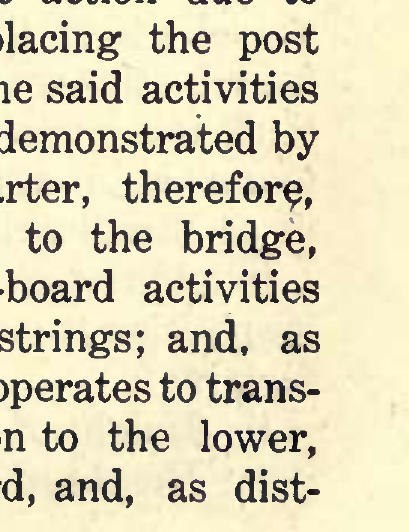
\includegraphics[width=0.8\textwidth]{../imagenes/pagina_309_fig_02.png}
\caption{Figura de la página 309}
\end{figure}

\section{VIOLIN TONE-PECULIARITIES.}

These facts unmistakably point to the risk in giving marked volume of tone to the new violin, because, such new violin is liable to suffer damag- ing loss of tone-power at what may be rightfully called premature age. From my viewpoint, it is much the wiser plan to slightly limit both distance and amplitude of transverse vibration and trust something to increasing flexibility of the wood in- evitably following use. [The work of Prof. Pietro Blaserna, Royal Uni- versity, Rome, is an admirable treatise for persons desiring study of sound in its relation to music.] POSITION OF THE POST: As the problem of the post has received various interpretations by different philosophers, and as no authoritative ground to stand upon appears in sight, therefore all persons are at liberty to hold and express opin- ions upon this question as suits themselves. Upon this basis, the following calculations are presented: As violin string-force depends upon augmenta- tion by normal and transverse vibration in the sounding-board, plus sympathetic action due to proximity of the strings, and, as placing the post below the bridge operates to confine said activities to the upper, right quarter, as is demonstrated by splitting up the lower, right quarter, therefore, position of the post, in its relation to the bridge, governs the location of sounding-board activities augmenting force of the A and E strings; and, as placing the post above the bridge operates to trans- fer normal and transverse vibration to the lower, right quarter of the sounding-board, and, as dist-

301

\begin{figure}[h!]
\centering

\includegraphics[width=0.8\textwidth]{../imagenes/pagina_310_fig_01.png}
\caption{Figura de la página 310}
\end{figure}

\begin{figure}[h!]
\centering
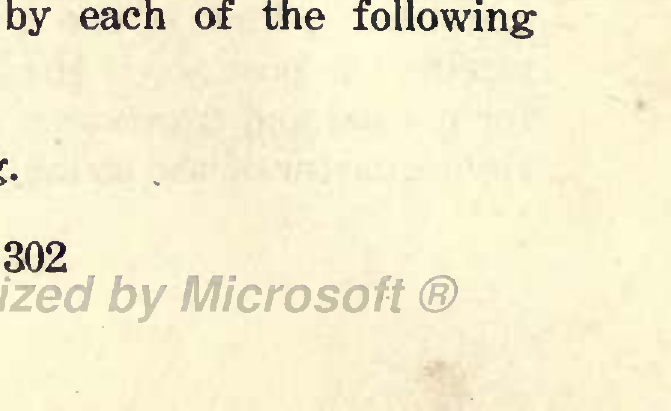
\includegraphics[width=0.8\textwidth]{../imagenes/pagina_310_fig_02.png}
\caption{Figura de la página 310}
\end{figure}

\begin{figure}[h!]
\centering
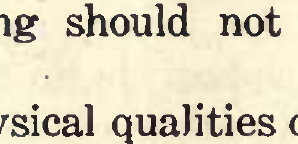
\includegraphics[width=0.8\textwidth]{../imagenes/pagina_310_fig_03.png}
\caption{Figura de la página 310}
\end{figure}

\begin{figure}[h!]
\centering
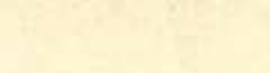
\includegraphics[width=0.8\textwidth]{../imagenes/pagina_310_fig_04.png}
\caption{Figura de la página 310}
\end{figure}

\section{VIOLIN TONE-PECULIARITIES.}

ance annihilates sympathetic action, therefore placing the post above the bridge operates to de- liver blows of diminished force upon contained air; hence diminished power of A and E-tone follows. As the influence of the post is chiefly exerted upon the A and E-strings, therefore, in selecting a posi- tion for the post, certain effects should be kept in view, as, greatest power of tone, and, best quality of tone. It happens quite often that greatest power of tone destroys best quality of tone; there- fore, in such case, a choice between greatest power and best quality of tone must be determined; and, in determining upon such choice, it is necessary to consider the post itself regardless of its position. This consideration is made necessary because such physical qualities in the post as length, dens- ity, and mass exert marked influence upon A and E-tone. Either of these attributes may defeat in- tention. Manifestly, preparatory training here be- comes of benefit, in fact, a necessity for securing best results in the work of post adjustment. As in all other matters pertaining to the modification of violin tone, the musical sense of the post-setter must be thrown into the balance; and, when such sense is a minus quantity, the failures following at- tempts at post-adjusting should not be charged up to Stradivarius. In addition to the physical qualities of the post, its position is modified by each of the following factors: 1. Height of bridge. 2. Height of arching.

302

\begin{figure}[h!]
\centering
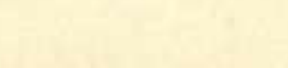
\includegraphics[width=0.8\textwidth]{../imagenes/pagina_311_fig_01.png}
\caption{Figura de la página 311}
\end{figure}

\begin{figure}[h!]
\centering

\includegraphics[width=0.8\textwidth]{../imagenes/pagina_311_fig_02.png}
\caption{Figura de la página 311}
\end{figure}

\begin{figure}[h!]
\centering

\includegraphics[width=0.8\textwidth]{../imagenes/pagina_311_fig_03.png}
\caption{Figura de la página 311}
\end{figure}

\begin{figure}[h!]
\centering
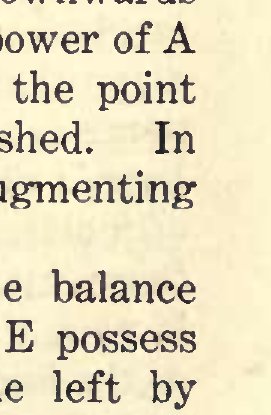
\includegraphics[width=0.8\textwidth]{../imagenes/pagina_311_fig_04.png}
\caption{Figura de la página 311}
\end{figure}

\begin{figure}[h!]
\centering
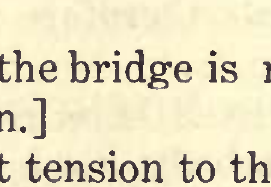
\includegraphics[width=0.8\textwidth]{../imagenes/pagina_311_fig_05.png}
\caption{Figura de la página 311}
\end{figure}

\begin{figure}[h!]
\centering
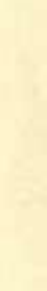
\includegraphics[width=0.8\textwidth]{../imagenes/pagina_311_fig_06.png}
\caption{Figura de la página 311}
\end{figure}

\begin{figure}[h!]
\centering
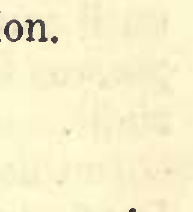
\includegraphics[width=0.8\textwidth]{../imagenes/pagina_311_fig_07.png}
\caption{Figura de la página 311}
\end{figure}

\begin{figure}[h!]
\centering
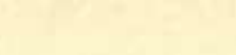
\includegraphics[width=0.8\textwidth]{../imagenes/pagina_311_fig_08.png}
\caption{Figura de la página 311}
\end{figure}

\begin{figure}[h!]
\centering
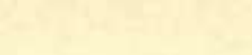
\includegraphics[width=0.8\textwidth]{../imagenes/pagina_311_fig_09.png}
\caption{Figura de la página 311}
\end{figure}

\section{VIOLIN TONE-PECULIARITIES.}

3. Thickness of plates at bridge-position. 4. Method of graduation. 5. Spring-quality of the plates. 6. Diameter and quality of string. Obviously, that position for the post securing greatest augmentation of A and E-tone can be de- termined only by trial. From differing methods for setting the post, the following is presented: Premising that length of the plates equals 14 inches, the bridge is first placed 8 inches from the upper end of the sounding-board for reasons here- tofore given. [This position for the bridge is modified by the method of graduation.] Applying sufficient tension to the strings to hold the bridge in position, set the post directly beneath the right foot of the bridge, and draw the strings up to either diapason normal, (international pitch, ) or up to concert pitch, thereafter maintaining the pitch and the gauge of strings decided upon. With the post in this position, observe the power of A and E-tone; then move the post downwards by 1-16 inch, and observe the increased power of A and E, and, continue thus until reaching the point where power of A and E. appears diminished. In returning the post to the point most augmenting power of A and E, move it by 1-32 inch. Upon reaching such point, observe the balance of power between A and E. , Should the E possess the greater power, move the post to the left by 1-32 inch, and observe the result; continuing thus

303

\begin{figure}[h!]
\centering
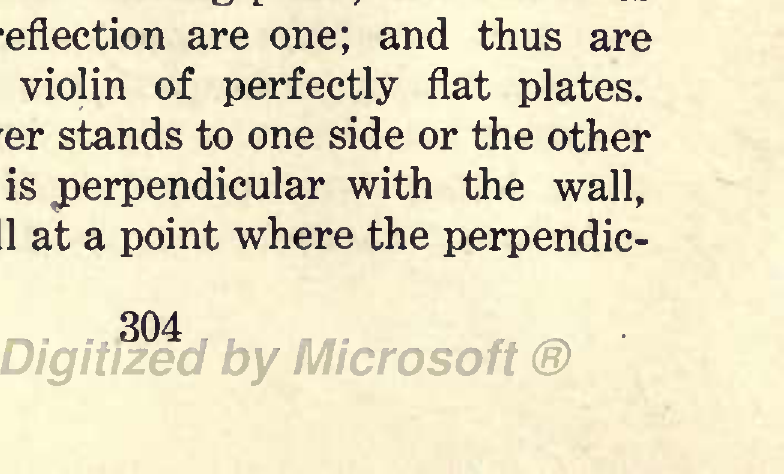
\includegraphics[width=0.8\textwidth]{../imagenes/pagina_312_fig_01.png}
\caption{Figura de la página 312}
\end{figure}

\begin{figure}[h!]
\centering
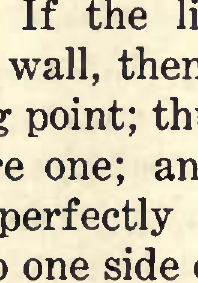
\includegraphics[width=0.8\textwidth]{../imagenes/pagina_312_fig_02.png}
\caption{Figura de la página 312}
\end{figure}

\begin{figure}[h!]
\centering
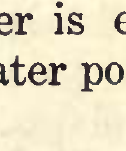
\includegraphics[width=0.8\textwidth]{../imagenes/pagina_312_fig_03.png}
\caption{Figura de la página 312}
\end{figure}

\begin{figure}[h!]
\centering
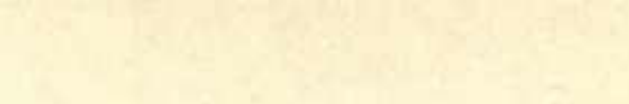
\includegraphics[width=0.8\textwidth]{../imagenes/pagina_312_fig_04.png}
\caption{Figura de la página 312}
\end{figure}

\section{VIOLIN TONE-PECULIARITIES.}

until equal power is established. Should the A possess the greater power, move the post to the right. In this work, defeat may follow from the follow- ing fact: With the diameter of the post equalling 3-16 inches, but slight deviation from the perpen- dicular causes the sounding-board to rest upon one or the other edge of the post. Thus, when the sounding-board rests upon the lower edge of the post, the distance from the bridge is practically 3-16 greater than appearances indicate; and as 1-32, more or less, causes perceptible effect upon A and E-string tone, therefore 6-32 becomes ample reason for defeat. ANGLES of INCIDENCE and REFLECTION, within the violin body, are important factors in the production of tone-intensity. The influence of these angles is easily comprehended; yet, in no form of arching whatever have these lines been definitely traced. These angles depend for existence upon a moving body and a solid reflecting surface, thus: The ball, thrown against the wall, travels along the line of incidence; and, as the ball rebounds, it travels along the line of reflection. If the line of inci- dence is perpendicular to the wall, then the ball re- bounds directly to its starting point; thus the lines of incidence and reflection are one; and thus are these lines in the violin of perfectly flat plates. If now, the thrower stands to one side or the other of the line which is perpendicular with the wall, and plants the ball at a point where the perpendic-

304

\begin{figure}[h!]
\centering

\includegraphics[width=0.8\textwidth]{../imagenes/pagina_313_fig_01.png}
\caption{Figura de la página 313}
\end{figure}

\begin{figure}[h!]
\centering

\includegraphics[width=0.8\textwidth]{../imagenes/pagina_313_fig_02.png}
\caption{Figura de la página 313}
\end{figure}

\section{VIOLIN TONE-PECULIARITIES.}

ular line touches the wall, then the ball will not rebound on the line of incidence nor upon the per- pendicular line, but will travel along a new line having precisely the same angle with the wall as the line of incidence; and thus are lines of sound- wave travel within the violin of arched plates. It is self-evident that such interior walls as turn sound-wave lines of travel away from the exits cause loss to intensity of tone; and per contra, such interior walls as direct sound-wave lines of travel toward the exits cause increased intensity of tone proportionate to the degree of concentration. Verbum sap First, establish the interior walls; later, the exterior walls. LABEL, VARNISH and PRICE vs SWEET TONE: Johann Holtzhammer is a herder of sheep. His summer home is on the mountain. From early morn till dewy eve, Johann listens to sweet sounds. The song of birds is sweet. The song of the rippling brook is sweet. The rustle of swaying boughs is sweet. The odor of pine is sweet. Even the noisy whirr of industry's wheels is bereft of the noise- wave ere it reaches up to Jo- hann's ears. At the base of detached rock, wild berries offer their sweet appearances and sweeter juices. The mountain air is sweet. The water in the rivulet is sweet. Indeed, life to Jo- hann is one round of sweetness; yet, Johann longs for something to keep his hands employed. With NATURE throbbing all around him, idleness be- comes oppressive. What would he do? What could he do? Make a violin? Why not? Here is

305

\begin{figure}[h!]
\centering
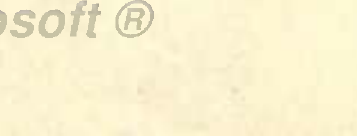
\includegraphics[width=0.8\textwidth]{../imagenes/pagina_314_fig_01.png}
\caption{Figura de la página 314}
\end{figure}

\begin{figure}[h!]
\centering

\includegraphics[width=0.8\textwidth]{../imagenes/pagina_314_fig_02.png}
\caption{Figura de la página 314}
\end{figure}

\begin{figure}[h!]
\centering

\includegraphics[width=0.8\textwidth]{../imagenes/pagina_314_fig_03.png}
\caption{Figura de la página 314}
\end{figure}

\begin{figure}[h!]
\centering
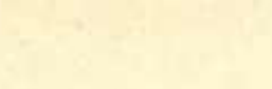
\includegraphics[width=0.8\textwidth]{../imagenes/pagina_314_fig_04.png}
\caption{Figura de la página 314}
\end{figure}

\begin{figure}[h!]
\centering
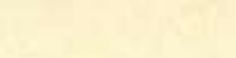
\includegraphics[width=0.8\textwidth]{../imagenes/pagina_314_fig_05.png}
\caption{Figura de la página 314}
\end{figure}

\section{VIOLIN TONE-PECULIARITIES.}

a fallen, giant pine. Yonder is a dead maple. There's the ax. Here's a jackknife. Where there's a will, there's a way. Those giant logs have been seasoning since Johann's grandsire herded the sheep; but, the ax is keen, and Jo- hann's jackknife is always ready for business. Time is nothing. Result is everything-. As Johann works, a nearby lark sings with undoubted approv- al. 'Tis true, Johann knows nothing of the Py- thagorean scale; nothing of the Palestrina scale; nothing of the piano, or temperate scale; nothing- of consonant overtones; nothing of harmonics a bassa; but, he does know sweet sound. 'Tis all he needs. Johann stains his violin with the juice of moun- tain berries.

Enough! Imitation is defied. The secret dies with Johann. The thrilling, enchanting, soulful, sweetly tend- er tone of Johann's violin had long been the cause for bird wonderment and worship prior to his passing; and, after his passing, each bird on that mountain vied with its neighbor in singing sweet and low upon the recurring date when Johann de- parted with his violin. Not one bird on that moun- tain ever mentioned the jackknifed angles upon Johann's violin; neither did Charon as Johann ap- plied for ferriage across the Styx; neither did the keeper of the great gate, as appears in the sequel. As Johann entered the long avenue, a multitude of shades with downcast mein, were standing at a

306

\begin{figure}[h!]
\centering

\includegraphics[width=0.8\textwidth]{../imagenes/pagina_315_fig_01.png}
\caption{Figura de la página 315}
\end{figure}

\begin{figure}[h!]
\centering
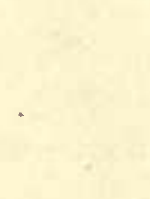
\includegraphics[width=0.8\textwidth]{../imagenes/pagina_315_fig_02.png}
\caption{Figura de la página 315}
\end{figure}

\begin{figure}[h!]
\centering
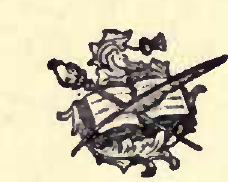
\includegraphics[width=0.8\textwidth]{../imagenes/pagina_315_fig_03.png}
\caption{Figura de la página 315}
\end{figure}

\begin{figure}[h!]
\centering
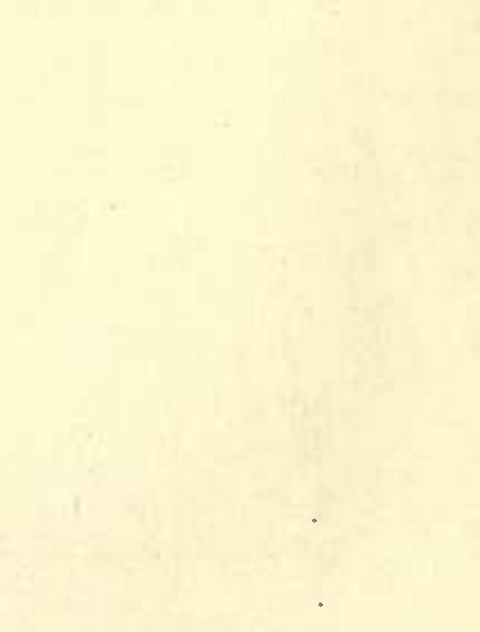
\includegraphics[width=0.8\textwidth]{../imagenes/pagina_315_fig_04.png}
\caption{Figura de la página 315}
\end{figure}

\begin{figure}[h!]
\centering
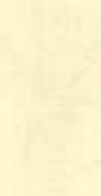
\includegraphics[width=0.8\textwidth]{../imagenes/pagina_315_fig_05.png}
\caption{Figura de la página 315}
\end{figure}

\begin{figure}[h!]
\centering
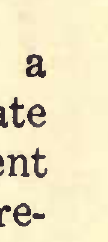
\includegraphics[width=0.8\textwidth]{../imagenes/pagina_315_fig_06.png}
\caption{Figura de la página 315}
\end{figure}

\begin{figure}[h!]
\centering
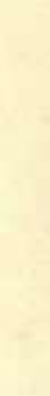
\includegraphics[width=0.8\textwidth]{../imagenes/pagina_315_fig_07.png}
\caption{Figura de la página 315}
\end{figure}

\begin{figure}[h!]
\centering
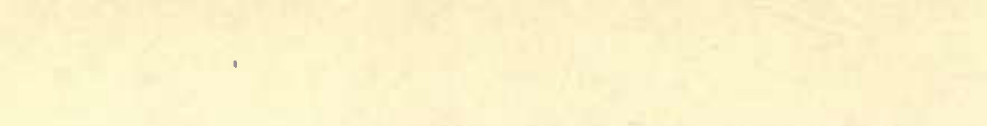
\includegraphics[width=0.8\textwidth]{../imagenes/pagina_315_fig_08.png}
\caption{Figura de la página 315}
\end{figure}

VIOLIN TONE-PECULIARITIES. halt upon either hand. Some of them bore ' 'mast- erpieces" upon which were conspicuous tickets lettered with the words, LABEL, and, VARNISH, and, a limited number bore conspicuous figures up- on the ticket, as, \$10,000, and, \$12,000. Although no affair of Johann's, yet, 'twas a wonderment whyfor such halting. As this gate keeper requires only the billionth part of a moment for computing the ad valorem in any invoice, there- fore, upon the instant Johann's immortal consign- ment arrived, the great gate swung open; and, in that brief interval, a glimpse of glory flashed down the long avenue; and, as the great gate closed be- hind Johann, there came up from the long avenue a sound as the gnashing of teeth.

307

\begin{figure}[h!]
\centering
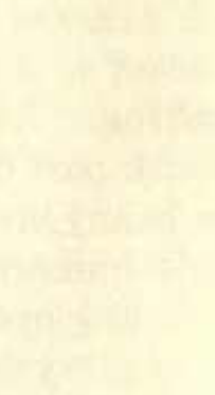
\includegraphics[width=0.8\textwidth]{../imagenes/pagina_316_fig_01.png}
\caption{Figura de la página 316}
\end{figure}

\begin{figure}[h!]
\centering
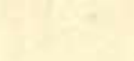
\includegraphics[width=0.8\textwidth]{../imagenes/pagina_316_fig_02.png}
\caption{Figura de la página 316}
\end{figure}

\$
